\documentclass[11pt, oneside]{article}   	% use "amsart" instead of "article" for AMSLaTeX format
\usepackage{geometry}                		% See geometry.pdf to learn the layout options. There are lots.
\geometry{letterpaper}                   		% ... or a4paper or a5paper or ... 
%\geometry{landscape}                		% Activate for for rotated page geometry
%\usepackage[parfill]{parskip}    		% Activate to begin paragraphs with an empty line rather than an indent
\usepackage{graphicx}				% Use pdf, png, jpg, or eps� with pdflatex; use eps in DVI mode
								% TeX will automatically convert eps --> pdf in pdflatex		
\usepackage{amssymb}
\usepackage{amsmath}
\usepackage{parskip}

\title{Cosine s+t quickly}
%\author{The Author}
\date{}							% Activate to display a given date or no date
\graphicspath{{/Users/telliott_admin/Dropbox/Tex/png/}}

\begin{document}
\section*{Cosine s+t quickly}
%\maketitle
%\section{}
%\subsection{}
\Large
If we consider a right triangle including angle $s$, we can scale the triangle to any size we like, and all the scaled triangles will be similar, with the third angle complementary to $s$, with sum equal to $\pi/2$.

Construct another right triangle containing angle $t$, and scale it so that the base adjacent to angle $t$ is just as long as the hypotenuse of the triangle containing angle $s$, and then draw them together as shown:
\begin{center} 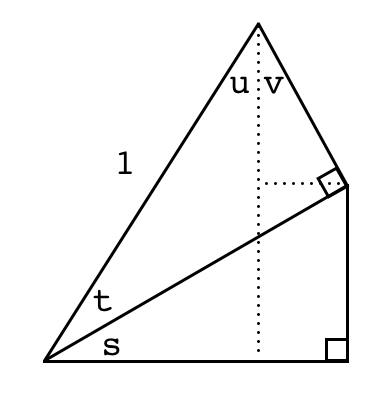
\includegraphics [scale=0.5] {sum_angle2.png} \end{center}
We have also scaled the joined triangles so that the hypotenuse of the second triangle has unit length.

Our crucial insight is to draw vertical and horizontal lines as shown.  Since the vertical line makes a right angle with the base, we have that:
\[ s + t + u = \frac{\pi}{2} =  t + u + v \]
\[ s = v \]
With some idea of what we are looking for, we write 
\[ \cos s + t = \cos s \cos t - \sin s \sin t \]
By $\cos s + t$ we really mean $\cos (s + t)$, but have left off the parentheses.

Our goal is to verify this eternal truth, using the diagram.  We add some labels to the sides of the triangles and substitute into the above equation, using the figure for reference:
\begin{center} 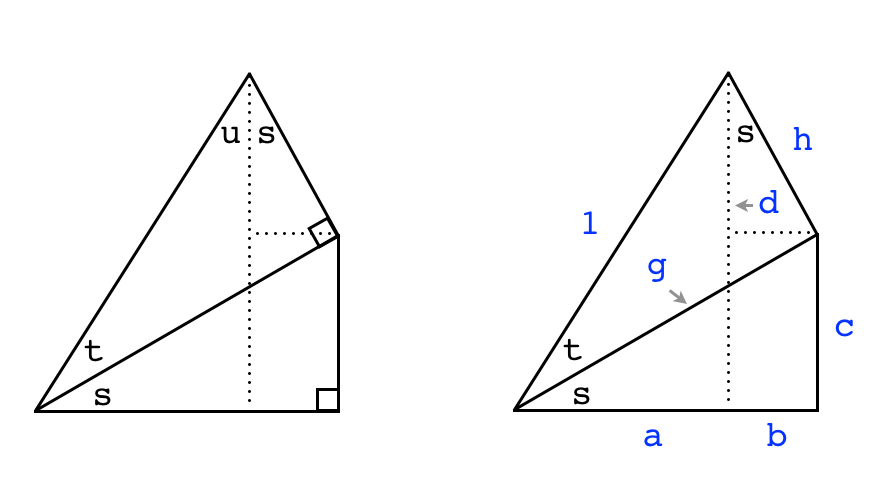
\includegraphics [scale=0.5] {sum_angle.png} \end{center}
From the figure
\[ \cos s = \frac{a+b}{g}; \ \ \ \cos t = \frac{g}{1}; \ \ \ \cos s \cos t = a + b \]
\[ \sin s = \frac{b}{h}; \ \ \ \sin t = \frac{h}{1}; \ \ \ \sin s \sin t = b \]
\[ \cos s + t = a = (a + b) - b \]
And from our calculation:
\[ \cos s \cos t - \sin s \sin t = (a + b) - b\]
Q.E.D.

\subsection*{extension to minus}
The first extension is to the difference $\cos s - t$.  We have
\[ \cos s + (-t) = \cos s \cos (-t) - \sin s \sin (-t) \]
Now, recall that $\cos -t = \cos t$ and $\sin -t = - \sin t$.  (Although it's not a proof, just visualize what happens near $\theta = 0$ and $\theta$ becomes negative).  Or, remember that the sine is an odd function $f(x) = - f(-x)$ and that the cosine is an even function.  Thus
\[ \cos s -t = \cos s \cos t + \sin s \sin t \]
I like this form because it's easy to verify that if $s=t$ then we have $\cos 0 = 1 = \cos^2 s + \sin^2 s = 1$, which is obviously correct.

\subsection*{extension to sine}
Referring back to the diagram (and again, with our goal clearly in mind)
\[ \sin s =  \frac{c}{g} \ \ \ \  \cos t = \frac{g}{1} \ \ \ \  \sin s \cos t = c  \]
\[ \sin t = \frac{h}{1} \ \ \ \  \cos s = \frac{d}{h} \ \ \ \ \sin t \cos s = d \]
But 
\[ \sin s + t = c + d =  \sin s \cos t +  \sin t \cos s \]

So ends the "quick" part.

\subsection*{alternative extension to sine}
Recall that the graphs of the sine and cosine follow the same pattern.  If we think of the angle $\theta$ as changing in time, the sine curve is delayed (shifted in phase) compared to the cosine.

It may be easier to think about particular values.  For the angle $\pi/2$, then $\sin \theta$ is a maximum.  The cosine was in the same position when the angle was $0$
\[ \cos 0 =  \sin \frac{\pi}{2} \]
or more generally
\[ \cos (\theta - \frac{\pi}{2}) = \sin \theta \]
On the other hand, if the angle is $-\pi/2$, then $\sin \theta$ is a minimum. The cosine was in the same position when the angle was $-\pi$
\[ \cos -\pi =  \sin -\frac{\pi}{2} \]
or more generally
\[ \sin (\theta - \frac{\pi}{2}) = \cos (\theta - \pi) =  -\cos \theta \]

These derivations are the hard part.

Returning to our result for the sum of the cosine, we had
\[ \cos (s + t) = \cos s \cos t - \sin s \sin t \]
Substitute $t - \pi/2$ for $t$ and obtain for the left-hand side
\[ \cos (s + t - \frac{\pi}{2} ) = \cos \ [ \ (s + t )- \frac{\pi}{2} \ ] \ = \sin (s + t ) \]
(think of $s+t$ as $\theta$ and compare with the first formula derived above).  So if we do the same manipulation on the right-hand side we can obtain an expression for $\sin s + t$.  

The first term on the right is easy, using the same formula it is just
\[ \cos s \cos (t - \frac{\pi}{2}) = \cos s \sin t \]
For the second term we have (using the second formula)
\[ - \sin s \sin (t - \frac{\pi}{2}) = - \sin s (- \cos t) = \sin s \cos t  \]
We have now
\[ \sin s + t  = \cos s \sin t + \sin s \cos t  \]


\end{document}  